\documentclass[a4paper,draft]{article}
\usepackage{scrextend}
%% for stopping floats
\usepackage{placeins}

%% Language and font encodings
\usepackage[english]{babel}
\usepackage[utf8x]{inputenc}
\usepackage[T1]{fontenc}
\usepackage[normalem]{ulem}
\useunder{\uline}{\ul}{}

%% Sets page size and margins
\usepackage[a4paper,top=3cm,bottom=2cm,left=3cm,right=3cm,marginparwidth=1.75cm,headheight=55pt]{geometry}

%% Useful packages
\usepackage{amsmath}
\usepackage{graphicx}

%% For todo 
\usepackage[pdftex,dvipsnames]{xcolor}  % Coloured text etc.
\usepackage[colorlinks=true, allcolors=blue]{hyperref}
\usepackage{xargs}                      % Use more than one optional parameter in a new commands
\usepackage[obeyDraft,colorinlistoftodos,prependcaption,textsize=tiny]{todonotes}
\newcommandx{\unsure}[2][1=]{\todo[linecolor=red,backgroundcolor=red!25,bordercolor=red,#1]{#2}}
\newcommandx{\change}[2][1=]{\todo[linecolor=blue,backgroundcolor=blue!25,bordercolor=blue,#1]{#2}}
\newcommandx{\info}[2][1=]{\todo[linecolor=OliveGreen,backgroundcolor=OliveGreen!25,bordercolor=OliveGreen,#1]{#2}}
\newcommandx{\improvement}[2][1=]{\todo[linecolor=Plum,backgroundcolor=Plum!25,bordercolor=Plum,#1]{#2}}
\newcommandx{\thiswillnotshow}[2][1=]{\todo[disable,#1]{#2}}
%% todo ends

%% for strike out, normalem
\usepackage[normalem]{ulem}
%% strike out ends

%% for line break in colorbox
\usepackage[]{tcolorbox}


%% no float table
\usepackage{float}
\restylefloat{table}

%% for header
%\usepackage{fancyhdr}

%%\usepackage[headheight=55pt]{geometry}

%\renewcommand{\headrulewidth}{2pt}
%\fancypagestyle{plain}{%
%  \fancyhead[L]{
%    \begin{tabular}{ll}
%%      \begin{tabular}[t]{c}
%        %\includegraphics[scale=0.3]{beeduck}%
%      \end{tabular} &
%      \begin{tabular}[b]{l}
%        \unsure{unsure} \change{change} \info{info} \improvement{improve}
%        Head of Department: The Bee Duck\tabularnewline
%        Vice chairmen: The Duck Bee\tabularnewline
%      \end{tabular}
%    \end{tabular}   
%  }%
%}

\pagestyle{plain}
%% end header

% for extra sub section
\usepackage{titlesec}
\titleclass{\subsubsubsection}{straight}[\subsection]

\newcounter{subsubsubsection}[subsubsection]
\renewcommand\thesubsubsubsection{\thesubsubsection.\arabic{subsubsubsection}}
\renewcommand\theparagraph{\thesubsubsubsection.\arabic{paragraph}} % optional; useful if paragraphs are to be numbered

\titleformat{\subsubsubsection}
  {\normalfont\normalsize\bfseries}{\thesubsubsubsection}{1em}{}
\titlespacing*{\subsubsubsection}
{0pt}{3.25ex plus 1ex minus .2ex}{1.5ex plus .2ex}

\makeatletter
\renewcommand\paragraph{\@startsection{paragraph}{5}{\z@}%
  {3.25ex \@plus1ex \@minus.2ex}%
  {-1em}%
  {\normalfont\normalsize\bfseries}}
\renewcommand\subparagraph{\@startsection{subparagraph}{6}{\parindent}%
  {3.25ex \@plus1ex \@minus .2ex}%
  {-1em}%
  {\normalfont\normalsize\bfseries}}
\def\toclevel@subsubsubsection{4}
\def\toclevel@paragraph{5}
\def\toclevel@paragraph{6}
\def\l@subsubsubsection{\@dottedtocline{4}{7em}{4em}}
\def\l@paragraph{\@dottedtocline{5}{10em}{5em}}
\def\l@subparagraph{\@dottedtocline{6}{14em}{6em}}
\makeatother

\setcounter{secnumdepth}{4}
\setcounter{tocdepth}{4}

% end e-s section

%% 	mind map 
%%\usepackage{epsfig}
\usepackage{tikz}
\usetikzlibrary{mindmap,backgrounds}
%% end mind map


\newcommand{\blap}[1]{\smash[b]{\begin{tabular}[t]{@{}c@{}}#1\end{tabular}}}

\title{Scene Analysis based Bluetooth Low Energy Indoor Positioning Methods\\ \textnormal{Master's Thesis Proposal} \textnormal{v0.4}}
\author{Srikanth Gadicherla}

\begin{document}
\maketitle
\renewcommand{\arraystretch}{1.5}
\thiswillnotshow{ \section{Abstract}
The thesis aims at getting a proof of concept for solutions to the \textbf{hybrid bluetooth low energy indoor positioning}(BLE-IP) along with \textbf{automatic node location identification}(ANOLI). ANOLI is mainly aimed during the calibration phase which gives out the locations of the bluetooth low energy(BLE) beacons. The BLE beacons are present inside the luminaires. The luminaires might either be installed in the ceiling or tethered to it. The location of BLE beacons determined using ANOLI and received signal strength indicator(RSSI) together are used in the BLE-IP task. The factors influencing the RSSI values is also studied and based on the target environment and accuracy the model is decided.  Simple applications like asset tracking is also implemented. }


\section{Goal of the thesis: Description}
\begin{enumerate}
\item \textbf{Automatic Node Location Identification(ANOLI):}
\begin{addmargin}[0em]{0em}% 1em left, 2em right
This task involves finding the locations of the beacons intelligently. Currently, Active Aheads, can read the RSSI values from all the other beacons, so, we need to employ an Machine Learning method for creating a topology of sensors. This task can also be named Self Organizing Sensor Network. The feasibility study is yet to be done but the main idea here is that combining the data from all the sensors and create a topology of sensors and get metadata out of it. This metadata would include to which cluster the particular sensor would belong to, clusters relative position to some landmark location, etc. \cite{raivisto} \\
So, we will have 2 weeks after the commissioning of the luminaires. 

\end{addmargin}

\item \textbf{Develop an algorithm for Bluetooth Low Energy Indoor Positioning(BLE-IP):}
\begin{addmargin}[0em]{0em}% 1em left, 2em right
In this task we want to find the position of a subject given the received signal strength indicator(RSSI) from the BLE beacons. This method would also make use of the information gained during the previous task. So, the idea here is that the metadata is loaded in to the mobile application, and when it starts reading the signal and it will relate the particular MAC(media access control) address to the topology and be used in the memory and non-memory methods. This metadata could also include the current sensor data, and the plan is to integrate as much data as possible for getting better accuracy. There is also conscious effort to make the application have less/no dependency on the internet. \\
The first task would be to understand the different biases via experiments so as to build a broad model which could be used in variety of environments. Then the different methods are deployed to check the accuracy based on that.\\

\textbf{Challenges:}
Need to deal with the different sampling frequencies of different AP's(BLE, WIFI) or smart-phone sensors in the algorithm [Check balzer82 github page or check Torres-Sospedra et al, 2.3, Para 2]
\end{addmargin}
\thiswillnotshow{
\item \textbf{Other tasks}:
\begin{enumerate}
\item \textbf{Applications:}
\begin{itemize}
\item \textbf{Asset tracking} could be accomplished. It includes a BLE device which sends out an advertisement signal which is read by the BLE devices in the mesh network for tracking its location. This is an inspiration\unsure{check this}  from Active Bat Localization System which uses Ultrasound\cite{hightower} \change{??} rather than bluetooth. Here, the bat is indoor mobile tags, similar to an asset.  
\end{itemize}
\item  \textbf{Pattern Recognition}: Another task would be to use the positioning data with other sensor data from smartphone over a period of time to learn spatial and temporal patterns\cite{he}. \info{check the IP\_LiFs\_MDS slides}
\
(Fingerprinting, radio map,..)
\end{enumerate}}

\end{enumerate}

\section{Introduction} \label{intro}
Indoor positioning(IP) is moving towards becoming ubiquitous and fulfilling the goal of Internet of Things(IoT) and Artificial Intelligence(AI) of Location Aware services\improvement{[cite here]}.  The explosion of usage of smartphones in the last decade has also enabled an exponential growth of this field. IP mainly leverages the sensor hub in smartphones like accelerometer, gyroscope, barometer, proximity, thermometer, pedometer, magnetic sensor, etc and wireless technologies like bluetooth and WiFi for accurately solving this problem. Signals of opportunities like magnetic field, pressure, light and sound intensity, Global Navigation Satellite System [Torres-Sospedra et al, A realistic evaluation of indoor positioning systems based on Wi-Fi fingerprinting, 2017], mobile network \cite{99} and frequency modulation(FM)\cite{98} signals have also been used which don't incur any additional infrastructure costs.  IP also gets impetus from interrelated fields like geo-location, augmented reality, natural user interface, gaming, man-machine interaction, and 3D mapping.

\vspace{3mm}
The need for indoor positioning arose because the traditional Global Positioning System(GPS) fares badly indoors due to signals attenuation and scattering caused by roofs and walls. This leads to higher uncertainty in estimation of location which sometimes spans across multiple rooms sabotaging the whole positioning problem. \improvement{put it to some other good place} Usage of indoor positioning(IP) can also be reasoned by following reasons \change{change the adjective here, not quite intuitive} condition, \unsure{right word?} convenience and commercialization. Condition in the sense people tend to stay indoors 90\% of the time according to Environment Protection Agency(EPA) \cite{geospatial}. Convenience as it can be used for locating rooms and tracking assets. Commercialization, in case of malls, groceries stores, can be used to send out discount coupons, personalized recommender engines. The positioning data could also be used to optimize the resource flow in hospitals or warehouse to minimize the operation cost\cite{max}.

\vspace{3mm}
Formally, the estimation of location of mobile unit(MU) using wireless technologies is called location sensing, geo-location, position location or radio-location\cite{liu}. The conventional GPS suffer with problems like building occlusion, multipath effect \cite{fang} and signal attenuation \cite{geospatial} \improvement{cite classic text book} indoors, and hence many other technologies have been advocated. \improvement{improve it} Even though the GPS technology can be improved using the GPS repeaters, the solution is not scalable and would require costly infrastructure. The new technologies for positioning include Assisted GPS, \thiswillnotshow{GPS + cellular mobile tower signal} Bluetooth Low Energy(BLE), MEMS sensors, LED, WiFi, Magnetic anomalies \unsure{is it fine if I use abbreviations directly} or methods used in conjunction with each other \cite{geospatial}. 

IP has been solved using the triangulation techniques like lateration with  time of arrival(TOA), time difference of arrival(TDOA), angle of arrival(AOA), received signal strength(RSS) or fingerprinting based scene analysis methods like decision based probabilistic method, k-Nearest Neighbour(k-NN), artificial neural networks(ANN) or proximity based methods\cite{liu} and Gaussian processes with latent variable models\cite{ferris}. For the rest of the article, we use beacons and nodes interchangeably. 
 \\

\info[inline]{ 
 1. AOA needs at least two known sources. 2. i-locate, open geo-data. \url{http://www.i-locate.eu/pilot-sites/}. 3. Before the advent of  bluetooth low energy(BLE) beacons, the indoor positioning was ....}

\subsection{Setup}
The BLE beacons are part intelligent luminaires are densely packed, the nodes can read the signal strengths from neighboring nodes. Generally, a location estimation task involves two hardware devices, one transmitting the signal and other receiving it\cite{liu}. Here, the transmitting device is bluetooth low energy chip(or WiFi router?) installed in Active Aheads. The other sensor data (there is no infrastructure for getting these data as of now),  follow-strength values is planned to be downloaded once and updated biweekly or monthly. The Active Aheads are part of a mesh network.
\chapter{Related work or Location Fingerprinting}

In this chapter, background on the indoor positioning methods would be presented. The chapter begins with the section \ref{2_rssi_data_analysis}, where in detailed discussion on data analysis of the RSSI values is provided. Section \ref{2_ind_pos} discusses the various methodology used previously. Section \ref{2_bayes_filter} talks how Bayesian Filters and Sequential Monte Carlo methods [\textbf{FixMe: should we add \ref{2_bayes_filter} and \ref{2_gp} to \ref{2_ind_pos}}]. Section \ref{2_bayes_filter} describes the Bayesian Filtering techniques. Section \ref{2_gp} provides the applications of Gaussian Processes and the state-of-the-art indoor positioning methods.

Before we start exploring the different methods for solving the indoor positioning problem, the initial challenge lies in getting the right data model as the RSSI values vary due to various external factors like [\textbf{FixMe: add factors here or refer to previous sections}]. 

The probabilistic nature of our positioning solution would allow seamless integration of inertial sensor data for increased performance.

%% Osan hienojaottelua alaosiin, eikä välttämättä edes tarpeen,
%% tässä vain esimerkkinä. Käytä harkintasi mukaan
%% osan jaottelua, joskus alaotsikot selventävät asioita ja
%% joskus vain sirpaloittavat tarpeettomasti tekstiä.
%%  Jaottelu menee seuraavasti:
%% \section{osan otsikko} 
%% \subsection{alaotsikko}
%% \subsubsection{ala-alaotsikko}
%% Tätä pitemälle ei pidä jaotella. 
%%
%% Three levels of hierarchy in sectioning should be enough

\section{Data Analysis of RSSI values} \label{2_rssi_data_analysis}

\section{Positioning Algorithms} \label{2_ind_pos}

The radio-signals based indoor positioning can be categorized as time-based, angle based and signal-strength based \citep{atia}

The indoor positioning algorithm's are usually mostly modeled either using Pathloss  or Gaussian process model. \fixme{add citation}

%%\begin{figure}[h!]
\centering
\begin{subfigure}{.5\textwidth}
  \centering
  \vspace*{1cm}
  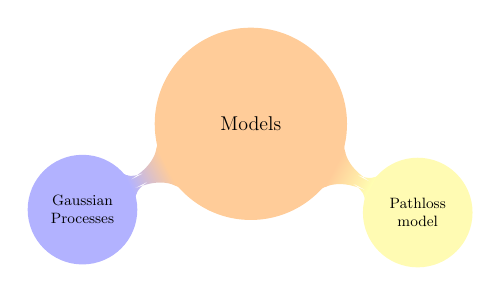
\begin{tikzpicture}[mindmap, grow cyclic, every node/.style=concept, concept color=orange!40,scale=0.6,transform shape,
	level 1/.append style={level distance=4cm,sibling angle=125}]
    \node{Models}[clockwise from=-28] 
    child [concept color=yellow!30]{ node (pmd) {Pathloss model}[clockwise from=-0]}
    child [concept color=blue!30]{ node (gp) {Gaussian Processes}[clockwise from=-260]}
    ;
  \end{tikzpicture}
  \label{fig:sub1}
\end{subfigure}%
\begin{subfigure}{.5\textwidth}
  \centering
  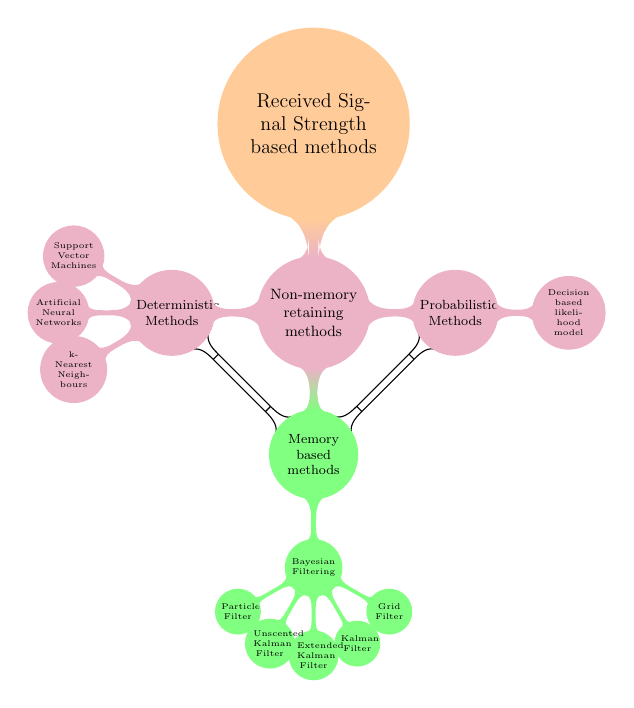
\begin{tikzpicture}[mindmap, grow cyclic, every node/.style=concept, concept color=orange!40,scale=0.6,transform shape,
	level 1/.append style={level distance=4cm,sibling angle=90},
    level 2/.append style={level distance=3cm,sibling angle=90}]
    
    \node{Received Signal Strength based methods}[clockwise from=-90] 
    
   child [concept color=purple!30] { node (nmem) {Non-memory retaining methods}[clockwise from=-0]
        child { node (pm) {Probabilistic Methods}[clockwise from=-0]
        		 child { node {Decision based likelihood model}}}
         child [concept color=green!50]{ node (mem) {Memory based methods}[clockwise from=-90]
        child { node {Bayesian Filtering}[clockwise from=-30]
        child { node {Grid Filter}}
         child { node {Kalman Filter}}
         child { node {Extended Kalman Filter}}
         child { node {Unscented Kalman Filter}}
         child{node {Particle Filter}}
        }}
        child { node (dm) {Deterministic Methods}[clockwise from=-150]
         child { node {k-Nearest Neighbours}}
         child { node {Artificial Neural Networks}}
         child { node {Support Vector Machines}}
         }
    };
    
    \begin{pgfonlayer}{background}
    \draw [circle connection bar]
       (mem) edge (dm)
       (pm) edge (mem);
  \end{pgfonlayer}
    



\end{tikzpicture}
  \label{fig:sub2}
\end{subfigure}
\caption{(left) Gaussian Processes and Pathloss models used in the thesis. (right) RSSI based methods used in the thesis. The colorless edges denote that memory based methods can be used in conjunction with non-memory based methods.}
\label{fig:test}
\end{figure}
%\FloatBarrier



\section{Bayesian Filtering} \label{2_bayes_filter}

%% esimerkki pakkotavutuksesta; "serif-tyyppinen" on tavutuksen kannalta
%% hankala, joten pakkotavutetaan se. 


%% Esimerkki taulukosta
\begin{table}[htb]
%% Taulukon teksti
        \caption{I'm your sample table \label{taulukko1}}
\begin{center}
\fbox{
\begin{tabular}{c|l|r}
\textbf{A} & 1 & $e^{j \omega t}$ \\ \hline
\textsf{B} & 2 & ${\mathfrak R}(c)$ \\ \hline
\texttt{C} & 3 & $ a \in \mathbb{A}$  
\end{tabular}
}
\end{center}
\end{table}

%% Jos käännät tämän tekstin pdflatex-komennolla ja tulostat sen katselu-
%% ohjelmasta, toteat todennäköisesti em. mittojen poikkeavan enemmän
%% kuin 1-2 mm. 
%% Tämä on seurausta pdf-tiedoston erilaisesta kirjaintyyppimäärityksestä.
%% Korkeatasoista painotyötä varten käytä vain latex-komentoa ja 
%% tulosta postscript-muotoon käännetystä tiedostosta. 
\section{Gaussian Processes} \label{2_gp}

Gaussian processes (GPs) are extensively used semi-parametric \footnote{going by the definition of basic GP, mean of Gaussian is non-parametric, but the conditional distribution is Gaussian, i.e, parametric.} modelling techniques 





\clearpage

\section{Work done}

\begin{enumerate}
\item Naive implementation of k-NN and GP measurement model for BLE based indoor positioning\cite{ble-ip-proj}.
\item Naive implementation of asset tracking using linear Pathloss model.
\item An smart-phone application for getting the RSSI values from the nodes. 
\end{enumerate}

\section{Methods and Materials}

\subsection{Methodology in the thesis}

The methods used in the thesis would be based on methods and models. Models could be either based on either Gaussian Processes(GP) or Pathloss model. Gaussian processes can be used both during the fingerprinting phase or as the measurement likelihood(or data) model. Pathloss model could be inaccurate as the signal suffers from multiple attenuations indoors so inclusion of prior knowledge is crucial here. So the pathloss model is used in conjunction with either GP as the mean function \cite{yiu}, some intelligent mapping between physical state space and signal space\cite{smailagic} or interpolation for improvement in the accuracy \cite{prasithsangaree}. 


\subsubsection{Different kinds of Methods} \label{methods}
\begin{enumerate}
\item \textbf{Non-memory based methods}:
These methods are deterministic or intelligent methods which try to relate the spatial space with the signal space. These methods are Trilateration/ Triangulation, k-Nearest Neighbors, Artificial Neural Networks etc. These methods estimate directly based on the RSSI values with no knowledge about the previous state or previous measurements, hence the name Non-memory based methods.
 
\item \textbf{Memory based methods (or Sequential Monte Carlo)}:
By adding a dynamic model or the prior to the non-memory based methods we arrive at Memory  based methods which are also called Sequential Monte Carlo based methods. The non-memory based methods are used as the measurement model, hence combining with the prior knowledge we arrive at the posterior or state estimate. There are different dynamic models used like stationary state model and constant velocity model(Bearing only Tracking; BOT) \cite{honkavirta}, the Augmented Coordinated Turn model could also be used to include the heading. Then, the sensor data like compass have to be include to get a better of this. 

Particle filters can be initialized using the location of node which gives highest RSSI \cite{honkavirta} value in conjunction with motion detection data using PIR sensors. And, also the particle filter could only be advanced when an event from the accelerometer is detected rather than updating it always \cite{torres-sospedra}. In other case, the particle states included the position, step length and heading offset with constant number of particles, so the individual particles were moved according to estimated step length and heading angle \cite{nurminen}. Calibrated Orientation sensor or compass for direction in which the person is moving\cite{torres-sospedra} shows that gyroscope and compass together can be used for this purpose.

\end{enumerate}

\begin{figure}[h!]
\centering
\begin{subfigure}{.5\textwidth}
  \centering
  \vspace*{1cm}
  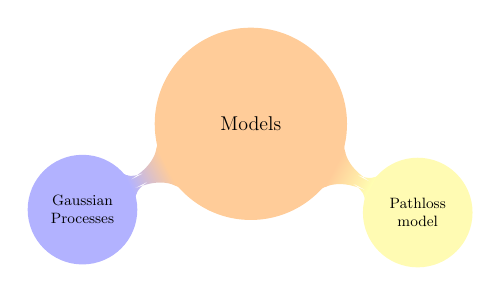
\begin{tikzpicture}[mindmap, grow cyclic, every node/.style=concept, concept color=orange!40,scale=0.6,transform shape,
	level 1/.append style={level distance=4cm,sibling angle=125}]
    \node{Models}[clockwise from=-28] 
    child [concept color=yellow!30]{ node (pmd) {Pathloss model}[clockwise from=-0]}
    child [concept color=blue!30]{ node (gp) {Gaussian Processes}[clockwise from=-260]}
    ;
  \end{tikzpicture}
  \label{fig:sub1}
\end{subfigure}%
\begin{subfigure}{.5\textwidth}
  \centering
  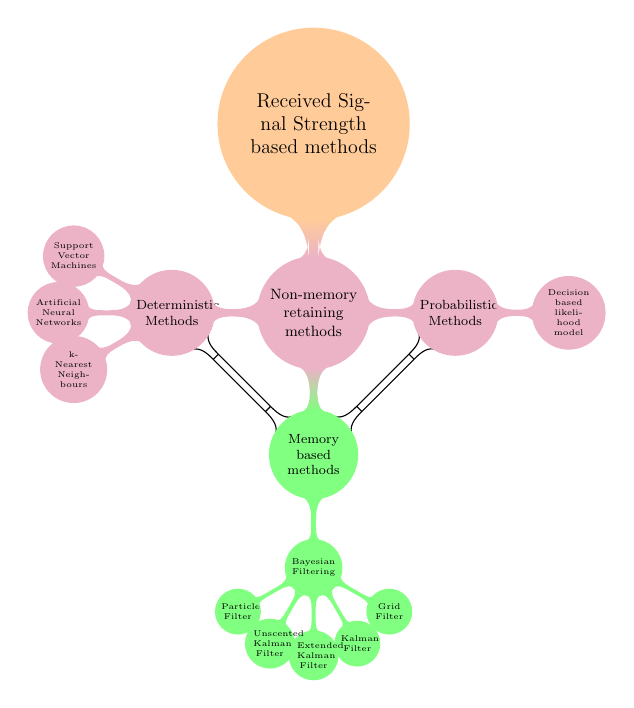
\begin{tikzpicture}[mindmap, grow cyclic, every node/.style=concept, concept color=orange!40,scale=0.6,transform shape,
	level 1/.append style={level distance=4cm,sibling angle=90},
    level 2/.append style={level distance=3cm,sibling angle=90}]
    
    \node{Received Signal Strength based methods}[clockwise from=-90] 
    
   child [concept color=purple!30] { node (nmem) {Non-memory retaining methods}[clockwise from=-0]
        child { node (pm) {Probabilistic Methods}[clockwise from=-0]
        		 child { node {Decision based likelihood model}}}
         child [concept color=green!50]{ node (mem) {Memory based methods}[clockwise from=-90]
        child { node {Bayesian Filtering}[clockwise from=-30]
        child { node {Grid Filter}}
         child { node {Kalman Filter}}
         child { node {Extended Kalman Filter}}
         child { node {Unscented Kalman Filter}}
         child{node {Particle Filter}}
        }}
        child { node (dm) {Deterministic Methods}[clockwise from=-150]
         child { node {k-Nearest Neighbours}}
         child { node {Artificial Neural Networks}}
         child { node {Support Vector Machines}}
         }
    };
    
    \begin{pgfonlayer}{background}
    \draw [circle connection bar]
       (mem) edge (dm)
       (pm) edge (mem);
  \end{pgfonlayer}
    



\end{tikzpicture}
  \label{fig:sub2}
\end{subfigure}
\caption{(left) Gaussian Processes and Pathloss models used in the thesis. (right) RSSI based methods used in the thesis. The colorless edges denote that memory based methods can be used in conjunction with non-memory based methods.}
\label{fig:test}
\end{figure}
%\FloatBarrier

\section{Plan}


\subsection{Experiments:} 

\subsubsection{Data Analysis of RSSI values.} \label{exp-rssi}
\begin{enumerate}
\item Different Biases in RSSI measurements
\begin{itemize}
\item User's presence and without user's presence.
\item Different phones.
\item Different orientation of phones, angles, height? 
\item Different material of luminaires.(metal, plastic, metal+plastic). Its an added bonus if we can get the different luminaire material information from the BLE signal.
\item Different orientation of BT chip (cardinal directions and upwards and downwards)
\item Different calibration time for fingerprinting.
\item Different calibration points.
\item Fingerprint measuring while being still, only in 4 cardinal positions and while rotating.
\end{itemize}
\item With nearest node not working.
\item Experiment with different orientation of the mobile device. Hypothesis is that the there is 5 dBm difference for the change in orientation \cite{kaemar}.
\end{enumerate}

\subsubsection{Methods} 
Next, based on the results of the experiments above implement the methods described in the \ref{methods}.

\thiswillnotshow{
\section{Observations:}
\begin{enumerate}
\item The signal strengths from the nodes
\end{enumerate}}

\FloatBarrier
\begin{table}[H]
\centering
\caption{Plan for the thesis}
\label{tab-plan}
\begin{tabular}{|l|l|l|}
\hline
\textbf{Month}                   & \textbf{Task}                      & \textbf{Remarks}                                                                           \\ \hline
February                         & REST API                  & Completed                                                                         \\ \hline
\textbf{Meeting 1}               & Slides:     &  \url{https://goo.gl/Up9ejx}                                                                                 \\ \hline
March                            & Literature Review         & \shortstack[l]{1. Made extensive notes of the reading \\2. Will move it to thesis \\ 3. Made plan.} \\ \hline
                                 & \textbf{Phase 1}          &                                                                                   \\ \hline
April \& May                      & Get better model:       & Influence of various biases; Experiment in \ref{exp-rssi}                         \\ \hline
June: week 23, 24                & Buffer period for 2 weeks & End of Phase 1                                                                    \\ \hline
                                 & \textbf{Phase 2}          &                                                                                   \\ \hline
\shortstack[l]{June: week 25, 26\\July: week 27} & Methods                   & Non-memory based methods. As discussed in \ref{methods}:                          \\ \hline
\shortstack[l]{July: rest \\August}              & Methods                   & Memory based methods                                                              \\ \hline
                                 & \textbf{Phase 3}          &                                                                                   \\ \hline
September                        & Writing                   & Compile results, write it to thesis, and survey paper.                         \\ \hline
October & \\Novemeber            & Writing                   & Polish the thesis,comments from instructor and supervisors.                       \\ \hline
\end{tabular}
\end{table}


















%\begin{figure}
%\centering
%\includegraphics[width=0.3\textwidth]{frog.jpg}
%\caption{\label{fig:frog}This frog was uploaded via the project menu.}
%\end{figure}

\begin{thebibliography}{9}

\bibitem{fang}
Yeqing Fang, Zhongliang Deng, Chen Xue, Jichao Jiao, Hui Zeng, Ruoyu Zheng, Shunbao Lu, “\textit{Application of an Improved K Nearest Neighbor Algorithm in WiFi Indoor Positioning},” China Satellite Navigation Conference(CSNC), 2015 Proceedings: Volume III2015342, Berlin, Germany, Springer 517524, Lecture Notes in Electrical Engineering, 10.1007/978-3-662-46632-$2\_45$, doi:10.1155/2014/649276



\bibitem{yuan}
Xianghui Yuan, Feng Lian, and Chongzhao Han, “\textit{Models and Algorithms for Tracking Target with Coordinated Turn Motion},” Mathematical Problems in Engineering, vol. 2014, Article ID 649276, 10 pages, 2014. doi:10.1155/2014/649276

\bibitem{liu}
H. Liu, H. Darabi, P. Banerjee and J. Liu, “\textit{Survey of Wireless Indoor Positioning Techniques and Systems},” IEEE Transactions on Systems, Man, and Cybernetics, Part C (Applications and Reviews), vol. 37, number 6, 1067-1080 pages, Nov 2007, doi:10.1109/TSMCC.2007.905750

\bibitem{yiu}
Yiu, H. Darabi, P. Banerjee and J. Liu, “\textit{Locating User Equipment and Access Points using RSSI fingerprints},” IEEE Transactions on Systems, Man, and Cybernetics, Part C (Applications and Reviews), vol. 37, number 6, 1067-1080 pages, Nov 2007, doi:10.1109/TSMCC.2007.905750

\bibitem{kamath}
Arjun. P. Kamath,"\textit{Indoor Location-Based Services In The Telecommunications Network}", Master Thesis, Department of Communications and Networking, School of Electrical Engineering, Aalto University, 2014.

\bibitem{ferris}
B. Ferris, D. Fox, and N. Lawrence. WiFi SLAM Using Gaussian Process Latent Variable Model. In JCAI, January 2007.
 
\bibitem{kontact}
Beacon, link: https://store.kontakt.io/our-products/30-double-battery-beacon.html.
 
\bibitem{max}
Discussion with Max Bj\"orkgren on 9th March.
 
\bibitem{martin}
Martin Sauter (2010). "3.7.1 Mobility Management in the Cell-DCH State". From GSM to LTE: An Introduction to Mobile Networks and Mobile Broadband (eBook). John Wiley \& Sons. p. 160. ISBN 9780470978221.

\bibitem{geospatial}
 http://www.geospatialworld.net/wp-content/uploads/magazine/Geospatial-World-August-2014.pdf.

\bibitem{raivisto}
 Discussion with Tommi Raivisto on 16th March.

\bibitem{ble-ip-proj}
 Project done for the course CS-E4030 - Seminar on Gaussian processes, School of Science, Aalto University.
 
\bibitem{he}
Suining He, S.-H. Gary Chan. \textit{"Wi-Fi Fingerprint-based Indoor Positioning:Recent Advances and Comparisons"}, IEEE Communications Surveys and Tutorials, 2015.

\bibitem{kaemar}
Kaemarungsi et al, Analysis of WLAN’s received signal strength indication for indoor location fingerprinting,2011

\bibitem{richter}
Philipp Richter, Revisiting Gaussian Process Regression Modeling for Localization in Wireless Sensor Networks, 2015.
 
 \bibitem{honkavirta}
 Honkarvirta et al, 2009; Prasithsangaree et al, 2002
 
 \bibitem{deluca}
 De Luca et al, Performance evaluation of Indoor Localization Techniques Based on RF Power measurements from Active or Passive Devices.
 
\bibitem{hightower}
Hightower et al, Location Sensing Techniques, A Technical report, 2001

\bibitem{mazzullah}
Mazzullah Khan et al,2017

\bibitem{umar}
Umar Ahmad, iBeacon Localization, Master Thesis.

\bibitem{smailagic}
Smailagic et al, 2002

\bibitem{prasithsangaree}
Prasithsangaree et al, 2002

\bibitem{torres-sospedra}
Torres-Sospedra et al, A realistic evaluation of indoor positioning systems based on Wi-Fi fingerprinting, 2017

\bibitem{nurminen}
Nurminen et al, Particle Filter and smoother for Indoor localization,2013

\end{thebibliography}


\end{document}